\documentclass[UTF8]{ctexart}

\setmainfont{Times New Roman}
% \setCJKmainfont{宋体}
% math bracket
%  ()
\newcommand{\brc}[1]{\left({{}#1}\right)}
%  []
\newcommand{\brm}[1]{\left[{{}#1}\right]}
%  ||
\newcommand{\brv}[1]{\left|{{}#1}\right|}
%  {}
\newcommand{\brf}[1]{\left\{{{}#1}\right\}}
%  ||
\newcommand{\brt}[1]{\left\Vert{{}#1}\right\Vert}
%  <>
\newcommand{\brg}[1]{\left<{{}#1}\right>}
%  floor
\newcommand{\floor}[1]{\lfloor{{}#1}\rfloor}
%  ceil
\newcommand{\ceil}[1]{\lceil{{}#1}\rceil}

% font
\newcommand{\fira}[1]{{\firacode {}#1}}

% abbr command
\newcommand{\ds}{\displaystyle}
\newcommand{\pt}{\partial}
\newcommand{\rint}[2]{\Big|^{{}#1}_{{}#2}}
\newcommand{\leg}{\left\lgroup}
\newcommand{\rig}{\right\rgroup}

% math symbol
\newcommand{\de}{\mathrm{d}}
\newcommand{\im}{\mathrm{im}}
\newcommand{\ord}{\mathrm{ord}}
\newcommand{\cov}{\mathrm{Cov}}
\newcommand{\lub}{\mathrm{LUB}}
\newcommand{\glb}{\mathrm{GLB}}
\newcommand{\var}{\mathrm{Var}}
\newcommand{\aut}{\mathrm{Aut}}
\newcommand{\sylow}{\mathrm{Sylow}}
\newcommand{\xhi}{\mathcal{X}}
\newcommand{\po}{\mathcal{P}}
\newcommand{\bi}{\mathrm{b}}
\newcommand{\rfl}{\mathcal{R}}

% algorithmic symbol
\newcommand{\gro}{\mathrm{O}}

% control command
\newcommand{\hfindent}{\hspace*{1em}}

\newfontfamily\firacode{Fira Code}
% \newfontfamily\firacode{Times New Roman}
% \newfontfamily\mincho{MS Mincho}

% math
\usepackage{ntheorem}
\usepackage{ulem}

\theoremseparator{ }
\newtheorem{dft}{Definition}
\newtheorem{tem}[dft]{Theorem}
\newtheorem{lem}[dft]{Lemma}
\newtheorem{epe}[dft]{Example}
\newtheorem{cor}[dft]{Corollary}

\usepackage{mathrsfs}
\usepackage{amsmath}
\usepackage{amssymb}
\usepackage{cancel}
%\usepackage{amsthm}

% control
\usepackage{ifthen}
\usepackage{intcalc}
\usepackage{array}

% format
\usepackage{indentfirst}
\usepackage{enumerate}
\usepackage{url}
\usepackage{setspace}

\usepackage{xcolor}

\definecolor{ballblue}{rgb}{0.13, 0.67, 0.8}
\definecolor{celestialblue}{rgb}{0.29, 0.59, 0.82}
\definecolor{bananayellow}{rgb}{1.0, 0.88, 0.21}
\definecolor{brilliantlavender}{rgb}{0.96, 0.73, 1.0}
\definecolor{burgundy}{rgb}{0.5, 0.0, 0.13}
\definecolor{cadmiumorange}{rgb}{0.93, 0.53, 0.18}
\definecolor{aqua}{rgb}{0.0, 1.0, 1.0}
\definecolor{auburn}{rgb}{0.43, 0.21, 0.1}
\definecolor{brass}{rgb}{0.71, 0.65, 0.26}
\definecolor{tangerine}{rgb}{0.95, 0.52, 0.0}
\definecolor{portlandorange}{rgb}{1.0, 0.35, 0.21}
\definecolor{mediumred-violet}{rgb}{0.73, 0.2, 0.52}
\definecolor{darkpastelpurple}{rgb}{0.59, 0.44, 0.84}

% listing set
\definecolor{func}{rgb}{0.29, 0.59, 0.82}
\definecolor{ftype}{rgb}{0.59, 0.44, 0.84}
\definecolor{cls}{rgb}{1.0, 0.35, 0.21}
\definecolor{slf}{rgb}{0.73, 0.2, 0.52}
\definecolor{backg}{HTML}{F7F7F7}
\definecolor{str}{HTML}{228B22}
% attestation
\definecolor{atte}{RGB}{178,34,34}

\usepackage{listings}

\lstset{
    backgroundcolor = \color{backg},
    basicstyle = \small,%
    escapeinside = ``,%
    keywordstyle = \color{func},% \underbar,%
    identifierstyle = {},%
    commentstyle = \color{blue},%
    stringstyle = \color{str}\ttfamily,%
    %labelstyle = \tiny,%
    extendedchars = false,%
    linewidth = \textwidth,%
}

\usepackage{geometry}

\geometry{
    left=2.0cm,
    right=2.0cm,
    top=2.5cm,
    bottom=2.5cm
}

\usepackage[
    colorlinks,
    linkcolor=blue,
    anchorcolor=blue,
    citecolor=blue
]{hyperref}

% table
\usepackage{csvsimple}
\usepackage{multirow}

% picture
\usepackage{graphicx}


% graph
\usepackage{tikz}
\usepackage{pgfplots}
\usetikzlibrary{
    quotes,
    angles,
    matrix,
    arrows,
    automata
}


\title{类C语言的词法分析器}
\author{Myriad Dreamin 2017211279 2017211301}
\date{}

\begin{document}
\setlength{\parindent}{2em}
%\renewcommand{\baselinestretch}{1.5}
\setlength{\baselineskip}{2.5em}
\maketitle
\subsection{要求}
\begin{enumerate}
	\item 可以识别出用C语言编写的源程序中的每个单词符号,并以记号的形式输出每个单词符号。
	\item 可以识别并跳过源程序中的注释。
	\item 可以统计源程序中的语句行数、各类单词的个数、以及字符总数,并输出统计结果。
	\item 检查源程序中存在的词法错误,并报告错误所在的位置。
	\item 对源程序中出现的错误进行适当的恢复,使词法分析可以继续进行,
	\item 对源程序进行一次扫描,即可检查并报告源程序中存在的所有词法
错误。
\end{enumerate}
\section{设计思路}
\subsection{组织策略}
如下是此次实验使用的结构体。
{\firacode
\begin{lstlisting}[language={[ANSI]C++}]  
template<typename stream_t, int64_t buffer_size, class Stream, bool unread_flag>
class Lexer {
private:
    using istream = std::basic_istream<stream_t>;
    using result_type = LexerResult<stream_t>;
    using string = std::basic_string<stream_t>;

    //`临时保存的字符串结果缓冲区`
    string buf;
    //`输入流`
    Stream program;
    //`LL(1)探针`
    stream_t nextToken;
    //`词法分析结果`
    result_type *result;

public:
    Lexer(istream &in);

    static result_type *new_result();

    // `词法分析入口`
    result_type *parse(result_type *result);
    
    // `自动机入口`
    bool parseMark();
    bool parseSpace();
    bool parseNumber();
    bool parseComment();
    bool parseKeywords();
    bool parseOperator();
    bool parseConstChar();
    bool parseIdentifier();
    bool parseConstString();

    bool emplaceDot();

private:
    void reclaim(const string &s);
    void set_buf(const string &s);
};
\end{lstlisting}
}
该类有4个成员,9个子自动机。parse为类的工作函数,parse根据nextToken探针选择进入不同的自动机转移。
\begin{figure}[!h]
    \centering
    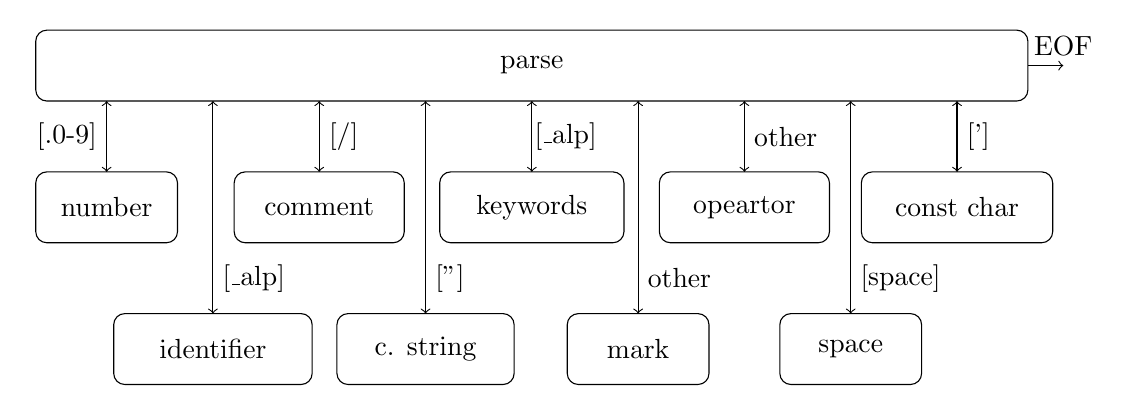
\begin{tikzpicture}[sibling distance=10em,
        every node/.style = {align=center}, scale=0.9]
    \node (N) at (0,0) {parse};
    \draw[rounded corners] (-7, -0.5) rectangle (7, 0.5);
    % \node (M) at (0,-3) {\fira{main}(go-back-n logic)};
    \draw[rounded corners] (-7, -1.5) rectangle (-5, -2.5);
    \draw[rounded corners] (-4.2, -1.5) rectangle (-1.8, -2.5);
    \draw[rounded corners] (-1.3, -1.5) rectangle (1.3, -2.5);
    \draw[rounded corners] (1.8, -1.5) rectangle (4.2, -2.5);
    \draw[rounded corners] (4.65, -1.5) rectangle (7.35, -2.5);
    \draw[rounded corners] (-5.9, -3.5) rectangle (-3.1, -4.5);
    \draw[rounded corners] (-2.75, -3.5) rectangle (-0.25, -4.5);
    \draw[rounded corners] (0.5, -3.5) rectangle (2.5, -4.5);
    \draw[rounded corners] (3.5, -3.5) rectangle (5.5, -4.5);

    \node at (-6,-2) {\fira{number}};
    \node at (-3,-2) {\fira{comment}};
    \node at (0,-2) {\fira{keywords}};
    \node at (3,-2) {\fira{opeartor}};
    \node at (6,-2) {\fira{const char}};
    \node at (-4.5,-4) {\fira{identifier}};
    \node at (-1.5,-4) {\fira{c. string}};
    \node at (1.5,-4) {\fira{mark}};
    \node at (4.5,-4) {\fira{space}};
    % \draw[rounded corners] (-7, -1.5) rectangle (-2, -2.5);
    % \node (S) at (4.5,-4) {\fira{receive\_buffer}};
    % \draw[rounded corners, loosely dashed] (7, -3.5) rectangle (2, -4.5);
    % \node at (0,-6) {\fira{put\_frame}};
    % \draw[rounded corners] (-7, -6.5) rectangle (7, -5.5);
    % \node at (0,-8) {Physical Layer};
    % \draw[rounded corners] (-7, -7.5) rectangle (7, -8.5);
    \draw[<->] (-6, -0.5) -- (-6, -1.5);
    \draw[<->] (-3, -0.5) -- (-3, -1.5);
    \draw[<->] (0, -0.5) -- (0, -1.5);
    \draw[<->] (3, -0.5) -- (3, -1.5);
    \draw[<->] (6, -0.5) -- (6, -1.5);
    \draw[<->] (-4.5, -0.5) -- (-4.5, -3.5);
    \draw[<->] (-1.5, -0.5) -- (-1.5, -3.5);
    \draw[<->] (1.5, -0.5) -- (1.5, -3.5);
    \draw[<->] (4.5, -0.5) -- (4.5, -3.5);
    \draw[->] (7, 0) -- (7.5, 0);
    \node[above] at (7.5, 0) {\fira{EOF}};
    \node[left] at (-6, -1) {\fira{[.0-9]}};
    \node[right] at (-3, -1) {\fira{[/]}};
    \node[right] at (-0.1, -1) {\fira{[\_alp]}};
    \node[right] at (3, -1) {\fira{other}};
    \node[right] at (6, -1) {\fira{[']}};
    \node[right] at (-4.5, -3) {\fira{[\_alp]}};
    \node[right] at (-1.5, -3) {\fira{["]}};
    \node[right] at (1.5, -3) {\fira{other}};
    \node[right] at (4.5, -3) {\fira{[space]}};    
    \end{tikzpicture}
\end{figure}
\par 将这些自动机从左至右,从上至下分别命名为$A_0=\mathcal{N}, A_1=\mathcal{C}, A_2=\mathcal{K}, A_3=\mathcal{O}, A_4=\mathcal{C}_{c},A_5=\mathcal{I}, A_6=\mathcal{C}_{s},A_7=\mathcal{S},A_8=\mathcal{M} $。
\par 那么总的自动机$A= (A_8\bigvee_{i=0}^7 A_{i})^*$。
\par 容易知道parse结点$n_0$相当于在9个自动机中担任$\epsilon$转移的$accept$和$fail$结点。
\par 为了方便,$n_0\xrightarrow{c}A_i$允许重合,但$c\neq \epsilon$。
\par 为了方便,$\mathcal{K}$和$\mathcal{O}$作为一组允许匹配的字符串集被组织成了Trie,在本实验中被命名为WordsFA,而其他自动机被命名为SerialFA。WordsFA的复杂度为$\Theta(n(1+\log |T|))$,$|T|$为字符集规模为一个常数(当然也可以牺牲空间优化为$\Theta(n)$),SerialFA的复杂度为$\Theta(n)$,所以$A$的复杂度为$\Theta(n)$。
\subsection{number自动机}
\begin{figure}[!h]
    \centering
    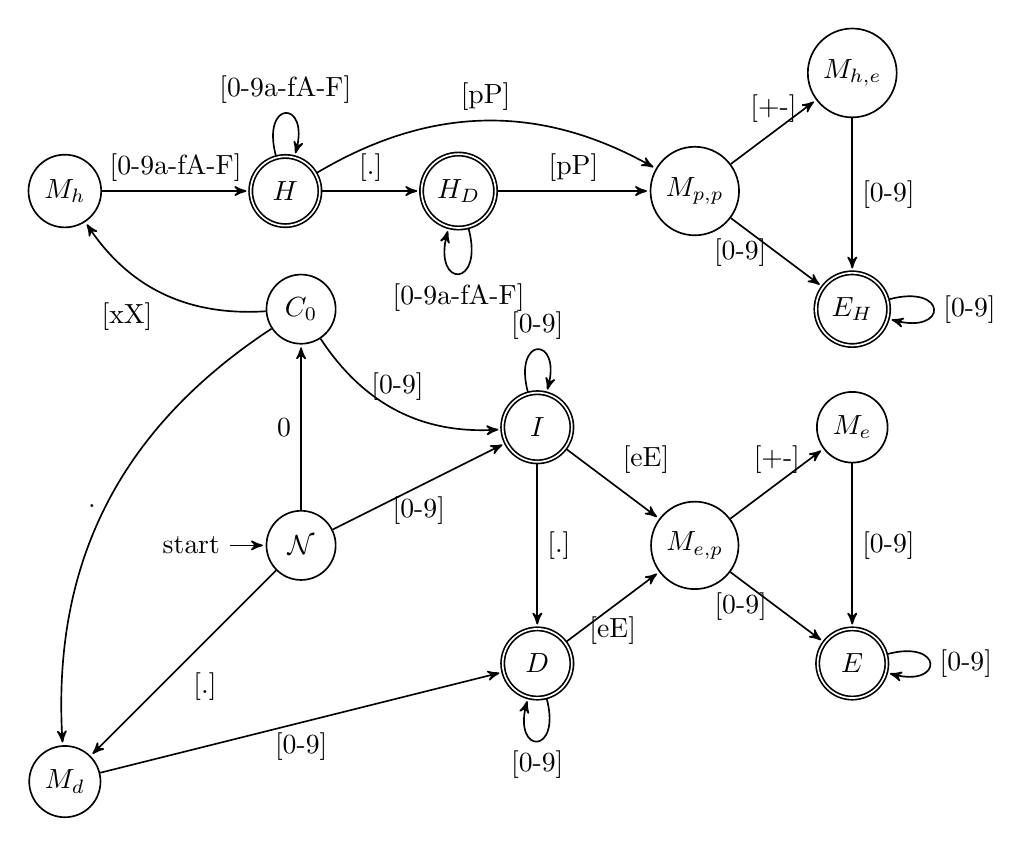
\begin{tikzpicture}[->,>=stealth',shorten >=1pt,auto,node distance=2.8cm,semithick]
    \tikzstyle{every state}=[shape=circle, rounded corners]

    \node[state, initial] (A) at (0, 0) {$\mathcal{N}$};
    \node[state] (C0) at (0, 3) {$C_0$};
    \node[state] (MD) at (-3, -3) {$M_d$};
    \node[state, accepting] (I) at (3, 1.5) {$I$};
    \node[state] (MH) at (-3, 4.5) {$M_h$};
    \node[state, accepting] (H) at (-0.2, 4.5) {$H$};
    \node[state, accepting] (HD) at (2, 4.5) {$H_D$};
    \node[state, accepting] (D) at (3, -1.5) {$D$};
    \node[state] (MEP) at (5, 0) {$M_{e,p}$};
    \node[state] (MPP) at (5, 4.5) {$M_{p,p}$};
    \node[state] (ME) at (7, 1.5) {$M_{e}$};
    \node[state, accepting] (E) at (7, -1.5) {$E$};
    \node[state] (MHE) at (7, 6) {$M_{h,e}$};
    \node[state, accepting] (HE) at (7, 3) {$E_H$};
    \path (A) edge node {0} (C0);
    \path (A) edge node {[.]} (MD);
    \path (A) edge node[below] {[0-9]} (I);
    \path (C0) edge[bend left] node {[xX]} (MH);
    \path (C0) edge[bend right] node [above] {[0-9]} (I);
    \path (C0) edge[bend right] node [left] {.} (MD);
    \path (MD) edge node [below] {[0-9]} (D);
    \path (I) edge [loop above] node {[0-9]} (I);
    \path (I) edge node {[.]} (D);
    \path (I) edge node {[eE]} (MEP);
    \path (MH) edge node {[0-9a-fA-F]} (H);
    \path (H) edge [loop above] node {[0-9a-fA-F]} (H);
    \path (HD) edge [loop below] node {[0-9a-fA-F]} (HD);
    \path (H) edge [bend left] node {[pP]} (MPP);
    \path (H) edge node {[.]} (HD);
    \path (HD) edge node {[pP]} (MPP);
    \path (D) edge [loop below] node {[0-9]} (D);
    \path (D) edge node [below] {[eE]} (MEP);
    \path (MEP) edge node [above] {[+-]} (ME);
    \path (MEP) edge node [left] {[0-9]} (E);
    \path (ME) edge node [right] {[0-9]} (E);
    \path (E) edge [loop right] node [right] {[0-9]} (E);
    \path (MPP) edge node [above] {[+-]} (MHE);
    \path (MPP) edge node [left] {[0-9]} (HE);
    \path (MHE) edge node [right] {[0-9]} (HE);
    \path (HE) edge [loop right] node [right] {[0-9]} (HE);
    \end{tikzpicture}
\end{figure}
\par 创建函数如下:
{\firacode
\begin{lstlisting}[language={[ANSI]C++}]
// ishex函数
static auto ishex = [](stream_t c) {
    return isdigit(c) || ('a' <= c && c <= 'f') || ('A' <= c && c <= 'F');
};
// 使用automaton命名空间
using namespace automaton;
// 使用线性有限状态
using fa_state = typename SerialFA<stream_t, raw_token_type, true>::fa_state;
// 创建自动机函数
static auto build_number_automaton = [&]() -> fa_state* {
    fa_state    *begin                   = fa_state::alloc(),
                *hex                     = 
                fa_state::alloc(static_cast<raw_token_type>(TokenType::NumberHex)),
                *integer                 = 
                fa_state::alloc(static_cast<raw_token_type>(TokenType::NumberInteger)),
                *decimal                 = 
                fa_state::alloc(static_cast<raw_token_type>(TokenType::NumberDecimal)),
                *hex_exponential         = 
            fa_state::alloc(static_cast<raw_token_type>(TokenType::NumberHexExponential)),
                *exponential             = 
                fa_state::alloc(static_cast<raw_token_type>(TokenType::NumberExponential)),
                *integer_or_maybe_others = 
                fa_state::alloc(static_cast<raw_token_type>(TokenType::NumberInteger)),
                *maybe_hex               = fa_state::alloc(),
                *maybe_integer           = fa_state::alloc(),
                *maybe_decimal           = fa_state::alloc(),
                *maybe_exp_accept_pm     = fa_state::alloc(),
                *maybe_exp               = fa_state::alloc(),
                *hex_decmial             = fa_state::alloc(),
                *maybe_hex_exp_accept_pm = fa_state::alloc(),
                *maybe_hex_exp           = fa_state::alloc();
    
    (*begin)
            >> std::make_pair('0', integer_or_maybe_others)
            >> std::make_pair('.', maybe_decimal)
            >> std::make_pair(isdigit, integer);

    (*integer_or_maybe_others)
            >> std::make_pair("xX", maybe_hex)
            >> std::make_pair('.', maybe_decimal)
            >> std::make_pair(isdigit, integer);
    
    (*integer)
            >> std::make_pair(isdigit, integer)
            >> std::make_pair('.', decimal)
            >> std::make_pair("eE", maybe_exp_accept_pm);
    
    (*maybe_hex)
            >> std::make_pair(ishex, hex);
    (*hex)  >> std::make_pair(ishex, hex)
            >> std::make_pair('.', hex_decmial)
            >> std::make_pair("pP", maybe_hex_exp_accept_pm);
    
    (*hex_decmial)
            >> std::make_pair(ishex, hex_decmial)
            >> std::make_pair("pP", maybe_hex_exp_accept_pm);
    (*maybe_hex_exp_accept_pm)
            >> std::make_pair("-+", maybe_hex_exp)
            >> std::make_pair(isdigit, hex_exponential);
    (*maybe_hex_exp)
            >> std::make_pair(isdigit, hex_exponential);
    (*hex_exponential)
            >> std::make_pair(isdigit, hex_exponential);

    (*maybe_decimal)
            >> std::make_pair(isdigit, decimal);
    (*decimal)
            >> std::make_pair(isdigit, decimal)
            >> std::make_pair("eE", maybe_exp_accept_pm);
    
    (*maybe_exp_accept_pm)
            >> std::make_pair("+-", maybe_exp)
            >> std::make_pair(isdigit, exponential);
    (*maybe_exp)
            >> std::make_pair(isdigit, exponential);
    (*exponential)
            >> std::make_pair(isdigit, exponential);
    

    return begin;
};
//创建自动机
static SerialFA<stream_t, raw_token_type, true> matcher(build_number_automaton);
\end{lstlisting}
}
\subsection{identifier自动机}
\begin{figure}[!h]
    \centering
    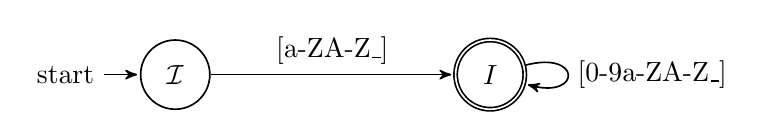
\begin{tikzpicture}[->,>=stealth',shorten >=1pt,auto,node distance=2.8cm,semithick]
    \tikzstyle{every state}=[shape=circle, rounded corners]

    \node[state, initial] (A) at (0, 0) {$\mathcal{I}$};
    \node[state, accepting] (I) at (4, 0) {$I$};
    \path (A) edge node {[a-ZA-Z\_]} (I);
    \path (I) edge [loop right] node {[0-9a-ZA-Z\_]} (I);
    \end{tikzpicture}
\end{figure}
\par 创建函数如下:
{\firacode
\begin{lstlisting}[language={[ANSI]C++}]
if (
    // `无先驱匹配, calI -> I`
    nextToken == '_' || isalpha(nextToken) ||
    // `从calK提升为I, calK -> I, 则还允许为数字`
    (buf.size() && isdigit(nextToken))) {
    
    buf.push_back(nextToken);
    nextToken = program.Read();

    // `I -> I`
    while(nextToken == '_' || isalnum(nextToken)) {
        buf.push_back(nextToken);
        nextToken = program.Read();
    }

    // `accept`
    result->register_token(TokenType::IdentifierType, buf);
    return true;
}

//如果允许回退
if (unread_flag) reclaim(buf);
return false;
\end{lstlisting}
}
\newpage
\subsection{comment自动机}
\begin{figure}[!h]
    \centering
    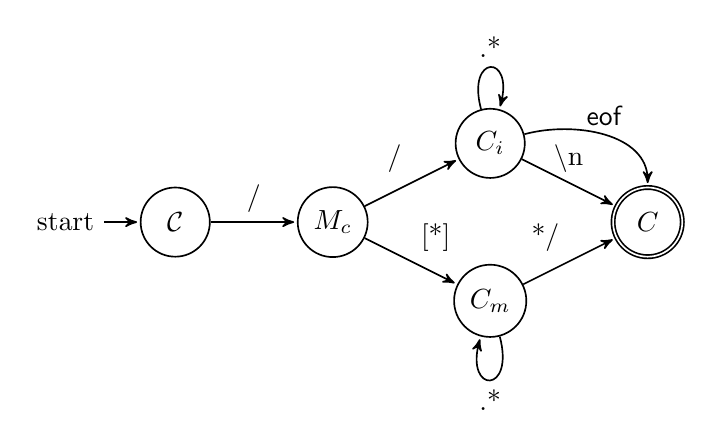
\begin{tikzpicture}[->,>=stealth',shorten >=1pt,auto,node distance=2.8cm,semithick]
    \tikzstyle{every state}=[shape=circle, rounded corners]

    \node[state, initial] (A) at (0, 0) {$\mathcal{C}$};
    \node[state] (MC) at (2, 0) {$M_c$};
    \node[state] (MCI) at (4, 1) {$C_i$};
    \node[state] (MCM) at (4, -1) {$C_m$};
    \node[state,accepting] (C) at (6, 0) {$C$};
    \path (A) edge node {/} (MC);
    \path (MC) edge node {/} (MCI);
    \path (MC) edge node {[*]} (MCM);
    \path (MCI) edge node [above] {\textbackslash n} (C);
    \path (MCI) edge[out=15, in=90] node [above] {$\mathsf{eof}$} (C);
    \path (MCM) edge node {*/} (C);
    \path (MCM) edge [loop below] node {.*} (MCM);
    \path (MCI) edge [loop above] node {.*} (MCI);
    \end{tikzpicture}
\end{figure}
\par 创建函数如下:
{\firacode
\begin{lstlisting}[language={[ANSI]C++}]
// `使用automaton命名空间`
using namespace automaton;
// `使用可回溯线性有限状态,至多回退一个字符`
using fa_state = typename SerialFA<stream_t, raw_token_type, true>::fa_state;
// `创建自动机函数`
static auto build_comment_automaton = [&]() -> fa_state* {
    fa_state    *begin         = fa_state::alloc(),
                *maybe_comment = fa_state::alloc(),
                *skipline      = fa_state::alloc(),
                *skiplines     = fa_state::alloc(),
                *accept        = 
                fa_state::alloc(static_cast<raw_token_type>(TokenType::CommentType));
    
    (*begin)
            >> std::make_pair('/', maybe_comment);
    
    (*maybe_comment)
            >> std::make_pair('/', skipline)
            >> std::make_pair('*', skiplines);
            
    (*skipline)
            >> std::make_pair(EOF, accept)
            >> fa_state::string(line_break, accept)
            >> std::make_pair(fa_state::any, skipline);
            
    (*skiplines)
            >> fa_state::string("*/", accept)
            >> std::make_pair(fa_state::any, skiplines);

    return begin;
};
//创建自动机
static SerialFA<stream_t, raw_token_type, true> matcher(build_comment_automaton);
\end{lstlisting}
}
\subsection{const string自动机}
\begin{figure}[!h]
    \centering
    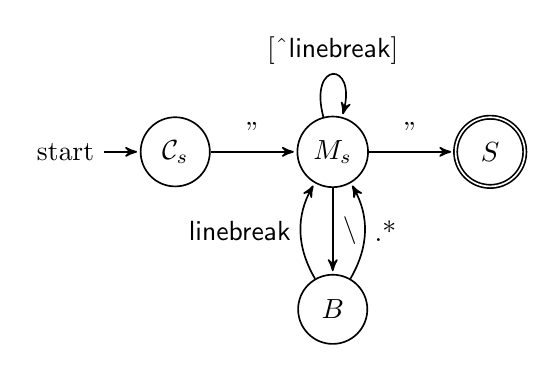
\begin{tikzpicture}[->,>=stealth',shorten >=1pt,auto,node distance=2.8cm,semithick]
    \tikzstyle{every state}=[shape=circle, rounded corners]

    \node[state, initial] (A) at (0, 0) {$\mathcal{C}_s$};
    \node[state] (MS) at (2, 0) {$M_s$};
    \node[state] (B) at (2, -2) {$B$};
    \node[state,accepting] (S) at (4, 0) {$S$};
    \path (A) edge node {\fira{"}} (MS);
    \path (MS) edge node {\fira{"}} (S);
    \path (MS) edge node {\textbackslash} (B);
    \path (MS) edge [loop above] node {[\textasciicircum$\mathsf{line break}$]} (MS);
    \path (B) edge [bend left] node {$\mathsf{line break}$} (MS);
    \path (B) edge [bend right] node [right] {.*} (MS);
    \end{tikzpicture}
\end{figure}
\par 创建函数如下:

{\firacode
\begin{lstlisting}[language={[ANSI]C++}]
// `line break 长度大于1时必须允许回溯`
static constexpr bool maybe_unread_flag = unread_flag || (line_break_length > 1);
// `使用automaton命名空间`
using namespace automaton;
// `使用线性有限状态`
using fa_state = typename SerialFA<stream_t, raw_token_type, maybe_unread_flag>::fa_state;
// `创建自动机函数`
static auto build_const_string_automaton = [&]() -> fa_state* {
    fa_state    *begin        = fa_state::alloc(),
                *maybe_string = fa_state::alloc(),
                *backslash    = fa_state::alloc(),
                *accept       =
                fa_state::alloc(static_cast<raw_token_type>(TokenType::ConstStringType));
    
    (*begin)
            >> std::make_pair('"', maybe_string);
    
    (*maybe_string)
            >> std::make_pair('\n', fa_state::discard)
            >> std::make_pair('\\', backslash)
            >> std::make_pair('"', accept)
            >> std::make_pair(fa_state::any, maybe_string);
            
    (*backslash)
            >> fa_state::string(line_break, maybe_string)
            >> std::make_pair(fa_state::any, maybe_string);

    return begin;
};
// `创建自动机`
static SerialFA<stream_t, raw_token_type, maybe_unread_flag>
    matcher(build_const_string_automaton);
\end{lstlisting}
}

\subsection{const char自动机}
\begin{figure}[!h]
    \centering
    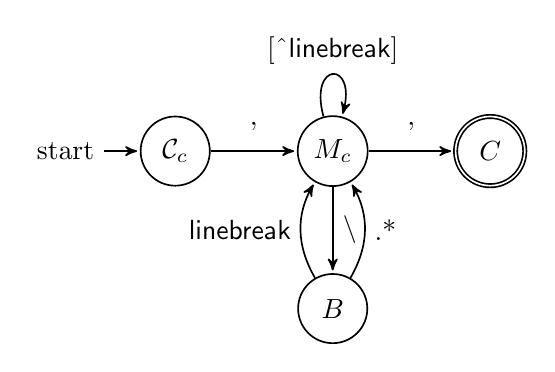
\begin{tikzpicture}[->,>=stealth',shorten >=1pt,auto,node distance=2.8cm,semithick]
    \tikzstyle{every state}=[shape=circle, rounded corners]

    \node[state, initial] (A) at (0, 0) {$\mathcal{C}_c$};
    \node[state] (MC) at (2, 0) {$M_c$};
    \node[state] (B) at (2, -2) {$B$};
    \node[state,accepting] (C) at (4, 0) {$C$};
    \path (A) edge node {\fira{'}} (MC);
    \path (MC) edge node {\fira{'}} (C);
    \path (MC) edge node {\textbackslash} (B);
    \path (MC) edge [loop above] node {[\textasciicircum$\mathsf{line break}$]} (MC);
    \path (B) edge [bend left] node {$\mathsf{line break}$} (MC);
    \path (B) edge [bend right] node [right] {.*} (MC);
    \end{tikzpicture}
\end{figure}
\par 创建函数如下:
{\firacode
\begin{lstlisting}[language={[ANSI]C++}]
// `line break 长度大于1时必须允许回溯`
static constexpr bool maybe_unread_flag = unread_flag || (line_break_length > 1);
// 使用automaton命名空间
using namespace automaton;
// 使用线性有限状态
using fa_state = typename SerialFA<stream_t, raw_token_type, maybe_unread_flag>::fa_state;
// 创建自动机函数
static auto build_const_char_automaton = [&]() -> fa_state* {
    fa_state    *begin        = fa_state::alloc(),
                *maybe_char   = fa_state::alloc(),
                *backslash    = fa_state::alloc(),
                *accept       =
                fa_state::alloc(static_cast<raw_token_type>(TokenType::ConstCharType));
    
    (*begin)
            >> std::make_pair('\'', maybe_char);
    
    (*maybe_char)
            >> std::make_pair('\n', fa_state::discard)
            >> std::make_pair('\\', backslash)
            >> std::make_pair('\'', accept)
            >> std::make_pair(fa_state::any, maybe_char);
            
    (*backslash)
            >> fa_state::string(line_break, maybe_char)
            >> std::make_pair(fa_state::any, maybe_char);

    return begin;
};
//创建自动机
static SerialFA<stream_t, raw_token_type, maybe_unread_flag> 
    matcher(build_const_char_automaton);
\end{lstlisting}
}
\subsection{mark自动机}
\begin{figure}[!h]
    \centering
    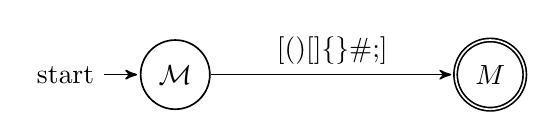
\begin{tikzpicture}[->,>=stealth',shorten >=1pt,auto,node distance=2.8cm,semithick]
    \tikzstyle{every state}=[shape=circle, rounded corners]

    \node[state, initial] (A) at (0, 0) {$\mathcal{M}$};
    \node[state, accepting] (M) at (4, 0) {$M$};
    \path (A) edge node {[()[]\{\}\#;]} (M);
    \end{tikzpicture}
\end{figure}
\par 创建函数如下:
{\firacode
\begin{lstlisting}[language={[ANSI]C++}]
for (raw_token_type i = 0; i < MarkRange; i++) {
    if (nextToken == _marks[i]) {
        result->register_token(static_cast<TokenType>(
            static_cast<raw_token_type>(TokenType::MarkBegin) + i));
        nextToken = program.Read();
        return true;
    }
}
\end{lstlisting}
}

\subsection{space自动机}
\begin{figure}[!h]
    \centering
    \begin{tikzpicture}[->,>=stealth',shorten >=1pt,auto,node distance=2.8cm,semithick]
    \tikzstyle{every state}=[shape=circle, rounded corners]

    \node[state, initial] (A) at (0, 0) {$\mathcal{S}$};
    \node[state, accepting] (S) at (4, 0) {$S$};
    \path (A) edge node {$\mathsf{space}$} (S);
    \path (I) edge [loop right] node {$\mathsf{space}$} (I);
    \end{tikzpicture}
\end{figure}
\par 创建函数如下:
{\firacode
\begin{lstlisting}[language={[ANSI]C++}]
if (isspace(nextToken)) {
    while(isspace(nextToken)) {
        nextToken = program.Read();
    }
    result->register_token(TokenType::SpaceType, " ");
    return true;
}
\end{lstlisting}
}
\subsection{keyword自动机和operator自动机}
由于$\mathcal{K}$和$\mathcal{O}$仅由字符串组成,所以组织成Trie进行匹配。

\section{程序测试}
输入测试如下
{\firacode
\begin{lstlisting}



tap
"1\
\
tup
extern fload f;
auto xx = y;
switch (xx) {
    case 3:
    static char a = '3';
    char a = '3'_wstring;
    const char *a = u""_rgba;
    default:
    do {
        for(long double float x=0;x<a;x++)if(a == '3') volatile a= 0.2; else a =/=*=^=|=&=-=
+=%=_=+-*/3, goto xxx;
    } while(a>3ll);
    break;
    return sizeof a;
    xxx:
    continue;
}

typedef enum t: register unsigned signed long long short int {A,B,C} T;
struct void enum {
    #define a = 0xffff, 0x, x, 00x, 0xg;
    union Union orz[] = a+b-c*d/e.a<<>>b->c>>=<<=d&?1.e1:~.e1!e1.e+1!1.e+1(^++t++++++-->=int
<=2<3!===&&|||%t);
}

1+2
"?????"
orz
""
"...
abdc
.1
.fff
'\n'
.1ff

``
0x00x0x
0x01ll
0x01
0x
0f
0x01.
0x01.p
0x01.p+
0x01.p+1
0x01.p1
0x01p+1
0x01l+1
0x01.+1
001.+1
01.+1
//
\end{lstlisting}
}

输出如下
{\firacode
\begin{lstlisting}[language={[ANSI]C++}]
LexerResult {
    code(NotMatch), error(5), lines(58), characters(769)
    [line, column](1,0), last(7128720), this(17002016, type(Space), content( ))
    [line, column](4,1), last(7091152), this(7091152, type(IdentifierType), name(tap))
    [line, column](5,0), last(17002016), this(7091280, type(Space), content( ))
    [line, column](5,1), last(7120112), this(7092176, type(Error)
error-line:<not revertable now, so cant anchor error on lines>
            ---------------------------------------------------
)
    [line, column](8,1), last(0), this(7091696, KeywordExtern)
    [line, column](8,7), last(7091280), this(7092272, type(Space), content( ))
    [line, column](8,8), last(7092224), this(7092224, type(IdentifierType), name(fload))
    [line, column](8,13), last(7092272), this(7092464, type(Space), content( ))
    [line, column](8,14), last(7121264), this(7091936, type(IdentifierType), name(f))
    [line, column](8,15), last(0), this(7091984, MarkSemicolon)
    [line, column](9,0), last(7092464), this(7091744, type(Space), content( ))
    [line, column](9,1), last(0), this(7092560, KeywordAuto)
    [line, column](9,5), last(7091744), this(7091792, type(Space), content( ))
    [line, column](9,6), last(17020464), this(7092320, type(IdentifierType), name(xx))
    [line, column](9,8), last(7091792), this(17020176, type(Space), content( ))
    [line, column](9,9), last(0), this(17020656, OperatorSimpleAssignment)
    [line, column](9,10), last(17020176), this(17019792, type(Space), content( ))
    [line, column](9,11), last(17020032), this(17020032, type(IdentifierType), name(y))
    [line, column](9,12), last(0), this(17019360, MarkSemicolon)
    [line, column](10,0), last(17019792), this(17019216, type(Space), content( ))
    [line, column](10,1), last(0), this(17020224, KeywordSwitch)
    [line, column](10,7), last(17019216), this(17020080, type(Space), content( ))
    [line, column](10,8), last(0), this(17019936, MarkLPAREN)
    [line, column](10,9), last(7092320), this(17020464, type(IdentifierType), name(xx))
    [line, column](10,11), last(0), this(17020416, MarkRPAREN)
    [line, column](10,12), last(17020080), this(17019408, type(Space), content( ))
    [line, column](10,13), last(0), this(17019504, MarkLBRACE)
    [line, column](11,0), last(17019408), this(17019072, type(Space), content( ))
    [line, column](11,5), last(0), this(17020320, KeywordCase)
    [line, column](11,9), last(17019072), this(17020560, type(Space), content( ))
    [line, column](11,10), last(7112848), this(17030128, type(NumberInteger), number(3))
    [line, column](11,12), last(0), this(17030224, OperatorConditionalSelector)
    [line, column](12,0), last(17020560), this(17030800, type(Space), content( ))
    [line, column](12,5), last(0), this(17029840, KeywordStatic)
    [line, column](12,11), last(17030800), this(17029264, type(Space), content( ))
    [line, column](12,12), last(0), this(17030560, KeywordChar)
    [line, column](12,16), last(17029264), this(17029456, type(Space), content( ))
    [line, column](12,17), last(7111088), this(17031040, type(IdentifierType), name(a))
    [line, column](12,18), last(17029456), this(17029744, type(Space), content( ))
    [line, column](12,19), last(0), this(17030752, OperatorSimpleAssignment)
    [line, column](12,20), last(17029744), this(17029504, type(Space), content( ))
    [line, column](12,21), last(7098800), this(17031088, type(ConstChar), content('3'))
    [line, column](12,24), last(0), this(17029600, MarkSemicolon)
    [line, column](13,0), last(17029504), this(17030320, type(Space), content( ))
    [line, column](13,5), last(0), this(17030368, KeywordChar)
    [line, column](13,9), last(17030320), this(17032688, type(Space), content( ))
    [line, column](13,10), last(17031040), this(17033840, type(IdentifierType), name(a))
    [line, column](13,11), last(17032688), this(17032640, type(Space), content( ))
    [line, column](13,12), last(0), this(17033408, OperatorSimpleAssignment)
    [line, column](13,13), last(17032640), this(17033600, type(Space), content( ))
    [line, column](13,14), last(17031088), this(17033456, type(ConstChar), content('3'))
    [line, column](13,17), last(17033360), this(17033360, type(IdentifierType), name(_wstring))
    [line, column](13,25), last(0), this(17033792, MarkSemicolon)
    [line, column](14,0), last(17033600), this(17034128, type(Space), content( ))
    [line, column](14,5), last(0), this(17034176, KeywordConst)
    [line, column](14,10), last(17034128), this(17034320, type(Space), content( ))
    [line, column](14,11), last(0), this(17033984, KeywordChar)
    [line, column](14,15), last(17034320), this(17033552, type(Space), content( ))
    [line, column](14,16), last(0), this(17034224, OperatorMultiplication)
    [line, column](14,17), last(17033840), this(17033216, type(IdentifierType), name(a))
    [line, column](14,18), last(17033552), this(17033648, type(Space), content( ))
    [line, column](14,19), last(0), this(17032784, OperatorSimpleAssignment)
    [line, column](14,20), last(17033648), this(17032448, type(Space), content( ))
    [line, column](14,21), last(17033696), this(17033696, type(IdentifierType), name(u))
    [line, column](14,22), last(7115728), this(17032592, type(ConstString), content(""))
    [line, column](14,24), last(17032976), this(17032976, type(IdentifierType), name(_rgba))
    [line, column](14,29), last(0), this(17033024, MarkSemicolon)
    [line, column](15,0), last(17032448), this(17033120, type(Space), content( ))
    [line, column](15,5), last(0), this(17033264, KeywordDefault)
    [line, column](15,12), last(0), this(17033168, OperatorConditionalSelector)
    [line, column](16,0), last(17033120), this(7096496, type(Space), content( ))
    [line, column](16,5), last(0), this(7095824, KeywordDo)
    [line, column](16,7), last(7096496), this(7096784, type(Space), content( ))
    [line, column](16,8), last(0), this(7095584, MarkLBRACE)
    [line, column](17,0), last(7096784), this(7096832, type(Space), content( ))
    [line, column](17,9), last(0), this(7095872, KeywordFor)
    [line, column](17,12), last(0), this(7095968, MarkLPAREN)
    [line, column](17,13), last(0), this(7097072, KeywordLong)
    [line, column](17,17), last(7096832), this(7096064, type(Space), content( ))
    [line, column](17,18), last(0), this(7096544, KeywordDouble)
    [line, column](17,24), last(7096064), this(7097120, type(Space), content( ))
    [line, column](17,25), last(0), this(7096928, KeywordFloat)
    [line, column](17,30), last(7097120), this(7096976, type(Space), content( ))
    [line, column](17,31), last(7121984), this(7095920, type(IdentifierType), name(x))
    [line, column](17,32), last(0), this(7096016, OperatorSimpleAssignment)
    [line, column](17,33), last(7121504), this(7096208, type(NumberInteger), number(0))
    [line, column](17,34), last(0), this(7096112, MarkSemicolon)
    [line, column](17,35), last(7095920), this(7096304, type(IdentifierType), name(x))
    [line, column](17,36), last(0), this(7096352, OperatorLT)
    [line, column](17,37), last(17033216), this(7095392, type(IdentifierType), name(a))
    [line, column](17,38), last(0), this(7096448, MarkSemicolon)
    [line, column](17,39), last(7096304), this(7097216, type(IdentifierType), name(x))
    [line, column](17,40), last(0), this(7096736, OperatorIncrement)
    [line, column](17,42), last(0), this(7095632, MarkRPAREN)
    [line, column](17,43), last(0), this(7096592, KeywordIf)
    [line, column](17,45), last(0), this(7095728, MarkLPAREN)
    [line, column](17,46), last(7095392), this(7096640, type(IdentifierType), name(a))
    [line, column](17,47), last(7096976), this(7095488, type(Space), content( ))
    [line, column](17,48), last(0), this(7098608, OperatorEQ)
    [line, column](17,50), last(7095488), this(7097696, type(Space), content( ))
    [line, column](17,51), last(17033456), this(7098800, type(ConstChar), content('3'))
    [line, column](17,54), last(0), this(7097456, MarkRPAREN)
    [line, column](17,55), last(7097696), this(7098368, type(Space), content( ))
    [line, column](17,56), last(0), this(7097408, KeywordVolatile)
    [line, column](17,64), last(7098368), this(7099040, type(Space), content( ))
    [line, column](17,65), last(7096640), this(7099232, type(IdentifierType), name(a))
    [line, column](17,66), last(0), this(7098848, OperatorSimpleAssignment)
    [line, column](17,67), last(7099040), this(7097792, type(Space), content( ))
    [line, column](17,68), last(7097552), this(7097552, type(NumberDecimal), number(0.2))
    [line, column](17,71), last(0), this(7098704, MarkSemicolon)
    [line, column](17,72), last(7097792), this(7097984, type(Space), content( ))
    [line, column](17,73), last(0), this(7098416, KeywordElse)
    [line, column](17,77), last(7097984), this(7099136, type(Space), content( ))
    [line, column](17,78), last(7099232), this(7099280, type(IdentifierType), name(a))
    [line, column](17,79), last(7099136), this(7098464, type(Space), content( ))
    [line, column](17,80), last(0), this(7098512, OperatorSimpleAssignment)
    [line, column](17,81), last(0), this(7098224, OperatorDivisionAssignment)
    [line, column](17,83), last(0), this(7098272, OperatorMultiplicationAssignment)
    [line, column](17,85), last(0), this(7098896, OperatorBitwiseXorAssignment)
    [line, column](17,87), last(0), this(7098992, OperatorBitwiseOrAssignment)
    [line, column](17,89), last(0), this(7101104, OperatorBitwiseAndAssignment)
    [line, column](17,91), last(0), this(7100672, OperatorSubtractionAssignment)
    [line, column](17,93), last(0), this(7100480, OperatorAdditionAssignment)
    [line, column](17,95), last(0), this(7101344, OperatorModuloAssignment)
    [line, column](17,97), last(7100384), this(7100384, type(IdentifierType), name(_))
    [line, column](17,98), last(0), this(7100192, OperatorSimpleAssignment)
    [line, column](17,99), last(0), this(7100864, OperatorAddition)
    [line, column](17,100), last(0), this(7099952, OperatorSubtraction)
    [line, column](17,101), last(0), this(7100000, OperatorMultiplication)
    [line, column](17,102), last(0), this(7100912, OperatorDivision)
    [line, column](17,103), last(17030128), this(7099616, type(NumberInteger), number(3))
    [line, column](17,104), last(0), this(7099760, OperatorComma)
    [line, column](17,105), last(7098464), this(7101200, type(Space), content( ))
    [line, column](17,106), last(0), this(7099712, KeywordGoto)
    [line, column](17,110), last(7101200), this(7101008, type(Space), content( ))
    [line, column](17,111), last(7103744), this(7101056, type(IdentifierType), name(xxx))
    [line, column](17,114), last(0), this(7100528, MarkSemicolon)
    [line, column](18,0), last(7101008), this(7099808, type(Space), content( ))
    [line, column](18,5), last(0), this(7100720, MarkRBRACE)
    [line, column](18,6), last(7099808), this(7100576, type(Space), content( ))
    [line, column](18,7), last(0), this(7101152, KeywordWhile)
    [line, column](18,12), last(0), this(7100096, MarkLPAREN)
    [line, column](18,13), last(7099280), this(7099472, type(IdentifierType), name(a))
    [line, column](18,14), last(0), this(7099520, OperatorGT)
    [line, column](18,15), last(7099616), this(7101296, type(NumberInteger), number(3))
    [line, column](18,16), last(7122656), this(7099568, type(IdentifierType), name(ll))
    [line, column](18,18), last(0), this(7100240, MarkRPAREN)
    [line, column](18,19), last(0), this(7100768, MarkSemicolon)
    [line, column](19,0), last(7100576), this(7099664, type(Space), content( ))
    [line, column](19,5), last(0), this(7100336, KeywordBreak)
    [line, column](19,10), last(0), this(7104128, MarkSemicolon)
    [line, column](20,0), last(7099664), this(7104176, type(Space), content( ))
    [line, column](20,5), last(0), this(7105376, KeywordReturn)
    [line, column](20,11), last(7104176), this(7105184, type(Space), content( ))
    [line, column](20,12), last(0), this(7103936, KeywordSizeof)
    [line, column](20,18), last(7105184), this(7103840, type(Space), content( ))
    [line, column](20,19), last(7099472), this(7104512, type(IdentifierType), name(a))
    [line, column](20,20), last(0), this(7105520, MarkSemicolon)
    [line, column](21,0), last(7103840), this(7103888, type(Space), content( ))
    [line, column](21,5), last(7101056), this(7103744, type(IdentifierType), name(xxx))
    [line, column](21,8), last(0), this(7103648, OperatorConditionalSelector)
    [line, column](22,0), last(7103888), this(7104848, type(Space), content( ))
    [line, column](22,5), last(0), this(7105232, KeywordContinue)
    [line, column](22,13), last(0), this(7105280, MarkSemicolon)
    [line, column](23,0), last(7104848), this(7104656, type(Space), content( ))
    [line, column](23,1), last(0), this(7103792, MarkRBRACE)
    [line, column](24,0), last(7104656), this(7104944, type(Space), content( ))
    [line, column](25,1), last(0), this(7104416, KeywordTypedef)
    [line, column](25,8), last(7104944), this(7105424, type(Space), content( ))
    [line, column](25,9), last(0), this(7103984, KeywordEnum)
    [line, column](25,13), last(7105424), this(7105040, type(Space), content( ))
    [line, column](25,14), last(7114768), this(7104032, type(IdentifierType), name(t))
    [line, column](25,15), last(0), this(7104560, OperatorConditionalSelector)
    [line, column](25,16), last(7105040), this(7104080, type(Space), content( ))
    [line, column](25,17), last(0), this(7103696, KeywordRegister)
    [line, column](25,25), last(7104080), this(7104272, type(Space), content( ))
    [line, column](25,26), last(0), this(7104320, KeywordUnsigned)
    [line, column](25,34), last(7104272), this(7106912, type(Space), content( ))
    [line, column](25,35), last(0), this(7107296, KeywordSigned)
    [line, column](25,41), last(7106912), this(7107200, type(Space), content( ))
    [line, column](25,42), last(0), this(7107248, KeywordLong)
    [line, column](25,46), last(7107200), this(7107344, type(Space), content( ))
    [line, column](25,47), last(0), this(7107392, KeywordLong)
    [line, column](25,51), last(7107344), this(7107056, type(Space), content( ))
    [line, column](25,52), last(0), this(7106720, KeywordShort)
    [line, column](25,57), last(7107056), this(7106048, type(Space), content( ))
    [line, column](25,58), last(0), this(7105712, KeywordInt)
    [line, column](25,61), last(7106048), this(7106864, type(Space), content( ))
    [line, column](25,62), last(0), this(7106000, MarkLBRACE)
    [line, column](25,63), last(7106624), this(7106624, type(IdentifierType), name(A))
    [line, column](25,64), last(0), this(7107152, OperatorComma)
    [line, column](25,65), last(7105856), this(7105856, type(IdentifierType), name(B))
    [line, column](25,66), last(0), this(7106192, OperatorComma)
    [line, column](25,67), last(7105760), this(7105760, type(IdentifierType), name(C))
    [line, column](25,68), last(0), this(7105808, MarkRBRACE)
    [line, column](25,69), last(7106864), this(7106096, type(Space), content( ))
    [line, column](25,70), last(7106144), this(7106144, type(IdentifierType), name(T))
    [line, column](25,71), last(0), this(7107440, MarkSemicolon)
    [line, column](26,0), last(7106096), this(7107488, type(Space), content( ))
    [line, column](26,1), last(0), this(7107536, KeywordStruct)
    [line, column](26,7), last(7107488), this(7106336, type(Space), content( ))
    [line, column](26,8), last(0), this(7107584, KeywordVoid)
    [line, column](26,12), last(7106336), this(7106432, type(Space), content( ))
    [line, column](26,13), last(0), this(7106576, KeywordEnum)
    [line, column](26,17), last(7106432), this(7110656, type(Space), content( ))
    [line, column](26,18), last(0), this(7108112, MarkLBRACE)
    [line, column](27,0), last(7110656), this(7108976, type(Space), content( ))
    [line, column](27,5), last(7092176), this(7110032, type(Error)
error-line:<not revertable now, so cant anchor error on lines>
            ---------------------------------------------------
)
    [line, column](27,6), last(7107872), this(7107872, type(IdentifierType), name(define))
    [line, column](27,12), last(7108976), this(7109936, type(Space), content( ))
    [line, column](27,13), last(7104512), this(7108736, type(IdentifierType), name(a))
    [line, column](27,14), last(7109936), this(7109984, type(Space), content( ))
    [line, column](27,15), last(0), this(7109696, OperatorSimpleAssignment)
    [line, column](27,16), last(7109984), this(7108688, type(Space), content( ))
    [line, column](27,17), last(7109360), this(7109360, type(NumberHex), number(0xffff))
    [line, column](27,23), last(0), this(7108208, OperatorComma)
    [line, column](27,24), last(7108688), this(7109024, type(Space), content( ))
    [line, column](27,25), last(7096208), this(7109648, type(NumberInteger), number(0))
    [line, column](27,26), last(7097216), this(7108160, type(IdentifierType), name(x))
    [line, column](27,27), last(0), this(7108304, OperatorComma)
    [line, column](27,28), last(7109024), this(7108352, type(Space), content( ))
    [line, column](27,29), last(7108160), this(7110464, type(IdentifierType), name(x))
    [line, column](27,30), last(0), this(7108400, OperatorComma)
    [line, column](27,31), last(7108352), this(7110176, type(Space), content( ))
    [line, column](27,32), last(7110224), this(7110224, type(NumberInteger), number(00))
    [line, column](27,34), last(7110464), this(7110512, type(IdentifierType), name(x))
    [line, column](27,35), last(0), this(7108448, OperatorComma)
    [line, column](27,36), last(7110176), this(7110080, type(Space), content( ))
    [line, column](27,37), last(7109648), this(7110128, type(NumberInteger), number(0))
    [line, column](27,38), last(7109408), this(7109408, type(IdentifierType), name(xg))
    [line, column](27,40), last(0), this(7110560, MarkSemicolon)
    [line, column](28,0), last(7110080), this(7110272, type(Space), content( ))
    [line, column](28,5), last(0), this(7108832, KeywordUnion)
    [line, column](28,10), last(7110272), this(7108880, type(Space), content( ))
    [line, column](28,11), last(7110320), this(7110320, type(IdentifierType), name(Union))
    [line, column](28,16), last(7108880), this(7109456, type(Space), content( ))
    [line, column](28,17), last(7115200), this(7109792, type(IdentifierType), name(orz))
    [line, column](28,20), last(0), this(7110416, MarkLSQUARE)
    [line, column](28,21), last(0), this(7109072, MarkRSQUARE)
    [line, column](28,22), last(7109456), this(7109120, type(Space), content( ))
    [line, column](28,23), last(0), this(7109552, OperatorSimpleAssignment)
    [line, column](28,24), last(7109120), this(7109888, type(Space), content( ))
    [line, column](28,25), last(7108736), this(7111328, type(IdentifierType), name(a))
    [line, column](28,26), last(0), this(7111232, OperatorAddition)
    [line, column](28,27), last(7113424), this(7111376, type(IdentifierType), name(b))
    [line, column](28,28), last(0), this(7111280, OperatorSubtraction)
    [line, column](28,29), last(7112272), this(7110800, type(IdentifierType), name(c))
    [line, column](28,30), last(0), this(7111472, OperatorMultiplication)
    [line, column](28,31), last(7114864), this(7110944, type(IdentifierType), name(d))
    [line, column](28,32), last(0), this(7111424, OperatorDivision)
    [line, column](28,33), last(7111984), this(7111520, type(IdentifierType), name(e))
    [line, column](28,34), last(0), this(7111568, OperatorMemberObject)
    [line, column](28,35), last(7111328), this(7111088, type(IdentifierType), name(a))
    [line, column](28,36), last(0), this(7111136, OperatorBitwiseLeftShift)
    [line, column](28,38), last(0), this(7111184, OperatorBitwiseRightShift)
    [line, column](28,40), last(7111376), this(7113424, type(IdentifierType), name(b))
    [line, column](28,41), last(0), this(7113280, OperatorMemberPointer)
    [line, column](28,43), last(7110800), this(7112272, type(IdentifierType), name(c))
    [line, column](28,44), last(0), this(7113472, OperatorBitwiseRightShiftAssignment)
    [line, column](28,47), last(0), this(7112032, OperatorBitwiseLeftShiftAssignment)
    [line, column](28,50), last(7110944), this(7114864, type(IdentifierType), name(d))
    [line, column](28,51), last(0), this(7112128, OperatorBitwiseAnd)
    [line, column](28,52), last(0), this(7111840, OperatorConditionalQuestionMark)
    [line, column](28,53), last(7113856), this(7113856, type(NumberExponential), number(1.e1))
    [line, column](28,57), last(0), this(7113904, OperatorConditionalSelector)
    [line, column](28,58), last(0), this(7114240, OperatorBitwiseNot)
    [line, column](28,59), last(0), this(7114288, OperatorMemberObject)
    [line, column](28,60), last(7113568), this(7114480, type(IdentifierType), name(e1))
    [line, column](28,62), last(0), this(7113376, OperatorLogicalNegation)
    [line, column](28,63), last(7114480), this(7113568, type(IdentifierType), name(e1))
    [line, column](28,65), last(0), this(7112224, OperatorMemberObject)
    [line, column](28,66), last(7111520), this(7111984, type(IdentifierType), name(e))
    [line, column](28,67), last(0), this(7112320, OperatorAddition)
    [line, column](28,68), last(7129728), this(7112368, type(NumberInteger), number(1))
    [line, column](28,69), last(0), this(7113616, OperatorLogicalNegation)
    [line, column](28,70), last(7114192), this(7114192, type(NumberExponential), number(1.e+1))
    [line, column](28,75), last(0), this(7112176, MarkLPAREN)
    [line, column](28,76), last(0), this(7112512, OperatorBitwiseXor)
    [line, column](28,77), last(0), this(7112704, OperatorIncrement)
    [line, column](28,79), last(7104032), this(7112080, type(IdentifierType), name(t))
    [line, column](28,80), last(0), this(7113952, OperatorIncrement)
    [line, column](28,82), last(0), this(7112464, OperatorIncrement)
    [line, column](28,84), last(0), this(7114000, OperatorIncrement)
    [line, column](28,86), last(0), this(7112560, OperatorDecrement)
    [line, column](28,88), last(0), this(7113664, OperatorGE)
    [line, column](28,90), last(0), this(7112656, KeywordInt)
    [line, column](28,93), last(0), this(7112608, OperatorLE)
    [line, column](28,95), last(7115392), this(7112752, type(NumberInteger), number(2))
    [line, column](28,96), last(0), this(7114096, OperatorLT)
    [line, column](28,97), last(7101296), this(7112848, type(NumberInteger), number(3))
    [line, column](28,98), last(0), this(7114576, OperatorNEQ)
    [line, column](28,100), last(0), this(7114336, OperatorEQ)
    [line, column](28,102), last(0), this(7112944, OperatorLogicalAnd)
    [line, column](28,104), last(0), this(7113808, OperatorLogicalInclusiveOr)
    [line, column](28,106), last(0), this(7114384, OperatorBitwiseOr)
    [line, column](28,107), last(0), this(7112896, OperatorModulus)
    [line, column](28,108), last(7112080), this(7114768, type(IdentifierType), name(t))
    [line, column](28,109), last(0), this(7113088, MarkRPAREN)
    [line, column](28,110), last(0), this(7113136, MarkSemicolon)
    [line, column](29,0), last(7109888), this(7114624, type(Space), content( ))
    [line, column](29,1), last(0), this(7114672, MarkRBRACE)
    [line, column](30,0), last(7114624), this(7114720, type(Space), content( ))
    [line, column](31,1), last(7112368), this(7111936, type(NumberInteger), number(1))
    [line, column](31,2), last(0), this(7114912, OperatorAddition)
    [line, column](31,3), last(7112752), this(7115392, type(NumberInteger), number(2))
    [line, column](32,0), last(7114720), this(7114960, type(Space), content( ))
    [line, column](32,1), last(7115056), this(7115056, type(ConstString), content("?????"))
    [line, column](33,0), last(7114960), this(7115104, type(Space), content( ))
    [line, column](33,1), last(7109792), this(7115200, type(IdentifierType), name(orz))
    [line, column](34,0), last(7115104), this(7115680, type(Space), content( ))
    [line, column](34,1), last(17032592), this(7115728, type(ConstString), content(""))
    [line, column](35,0), last(7115680), this(7115008, type(Space), content( ))
    [line, column](35,1), last(7110032), this(7115536, type(Error)
error-line:<not revertable now, so cant anchor error on lines>
            ---------------------------------------------------
)
    [line, column](36,1), last(7123424), this(7123424, type(IdentifierType), name(abdc))
    [line, column](37,0), last(7115008), this(7123520, type(Space), content( ))
    [line, column](37,1), last(7123376), this(7123616, type(NumberDecimal), number(.1))
    [line, column](38,0), last(7123520), this(7123136, type(Space), content( ))
    [line, column](38,1), last(0), this(7123952, OperatorMemberObject)
    [line, column](38,2), last(7123664), this(7123664, type(IdentifierType), name(fff))
    [line, column](39,0), last(7123136), this(7123712, type(Space), content( ))
    [line, column](39,1), last(7123328), this(7123328, type(ConstChar), content('\n'))
    [line, column](40,0), last(7123712), this(7123808, type(Space), content( ))
    [line, column](40,1), last(7123616), this(7123376, type(NumberDecimal), number(.1))
    [line, column](40,3), last(7122512), this(7122512, type(IdentifierType), name(ff))
    [line, column](41,0), last(7123808), this(7122176, type(Space), content( ))
    [line, column](42,1), last(7115536), this(7122224, type(Error)
error-line:<not revertable now, so cant anchor error on lines>
            ---------------------------------------------------
)
    [line, column](42,2), last(7122224), this(7120112, type(Error)
error-line:<not revertable now, so cant anchor error on lines>
            ---------------------------------------------------
)
    [line, column](43,0), last(7122176), this(7122848, type(Space), content( ))
    [line, column](43,1), last(7121936), this(7121936, type(NumberHex), number(0x00))
    [line, column](43,5), last(7121168), this(7121168, type(IdentifierType), name(x0x))
    [line, column](44,0), last(7122848), this(7120544, type(Space), content( ))
    [line, column](44,1), last(7131408), this(7122992, type(NumberHex), number(0x01))
    [line, column](44,5), last(7099568), this(7122656, type(IdentifierType), name(ll))
    [line, column](45,0), last(7120544), this(7120592, type(Space), content( ))
    [line, column](45,1), last(7122992), this(7122896, type(NumberHex), number(0x01))
    [line, column](46,0), last(7120592), this(7121216, type(Space), content( ))
    [line, column](46,1), last(7110128), this(7123040, type(NumberInteger), number(0))
    [line, column](46,3), last(7110512), this(7121984, type(IdentifierType), name(x))
    [line, column](47,0), last(7121216), this(7123088, type(Space), content( ))
    [line, column](47,1), last(7123040), this(7121504, type(NumberInteger), number(0))
    [line, column](47,3), last(7091936), this(7121264, type(IdentifierType), name(f))
    [line, column](48,0), last(7123088), this(7120832, type(Space), content( ))
    [line, column](48,1), last(7122896), this(7122560, type(NumberHex), number(0x01))
    [line, column](48,6), last(0), this(7120640, OperatorMemberObject)
    [line, column](49,0), last(7120832), this(7120688, type(Space), content( ))
    [line, column](49,1), last(7122560), this(7122944, type(NumberHex), number(0x01))
    [line, column](49,6), last(0), this(7120448, OperatorMemberObject)
    [line, column](49,8), last(7120304), this(7120160, type(IdentifierType), name(p))
    [line, column](50,0), last(7120688), this(7120208, type(Space), content( ))
    [line, column](50,1), last(7122944), this(7122032, type(NumberHex), number(0x01))
    [line, column](50,6), last(0), this(7120256, OperatorMemberObject)
    [line, column](50,7), last(7120160), this(7120304, type(IdentifierType), name(p))
    [line, column](50,8), last(0), this(7121072, OperatorAddition)
    [line, column](51,0), last(7120208), this(7120400, type(Space), content( ))
    [line, column](51,1), last(7120784), this(7120784, type(NumberHexExponential), number(0x01.p+1))
    [line, column](52,0), last(7120400), this(7121312, type(Space), content( ))
    [line, column](52,1), last(7121408), this(7121408, type(NumberHexExponential), number(0x01.p1))
    [line, column](53,0), last(7121312), this(7121744, type(Space), content( ))
    [line, column](53,1), last(7131552), this(7131552, type(NumberHexExponential), number(0x01p+1))
    [line, column](54,0), last(7121744), this(7132176, type(Space), content( ))
    [line, column](54,1), last(7122032), this(7132080, type(NumberHex), number(0x01))
    [line, column](54,5), last(7131840), this(7131840, type(IdentifierType), name(l))
    [line, column](54,6), last(0), this(7131888, OperatorAddition)
    [line, column](54,7), last(7111936), this(7132224, type(NumberInteger), number(1))
    [line, column](55,0), last(7132176), this(7131456, type(Space), content( ))
    [line, column](55,1), last(7132080), this(7131408, type(NumberHex), number(0x01))
    [line, column](55,5), last(0), this(7131360, OperatorMemberObject)
    [line, column](55,6), last(0), this(7132128, OperatorAddition)
    [line, column](55,7), last(7132224), this(7131696, type(NumberInteger), number(1))
    [line, column](56,0), last(7131456), this(7129536, type(Space), content( ))
    [line, column](56,1), last(7128576), this(7128576, type(NumberDecimal), number(001.))
    [line, column](56,5), last(0), this(7130352, OperatorAddition)
    [line, column](56,6), last(7131696), this(7130304, type(NumberInteger), number(1))
    [line, column](57,0), last(7129536), this(7130160, type(Space), content( ))
    [line, column](57,1), last(7128960), this(7128960, type(NumberDecimal), number(01.))
    [line, column](57,4), last(0), this(7129632, OperatorAddition)
    [line, column](57,5), last(7130304), this(7129728, type(NumberInteger), number(1))
    [line, column](58,0), last(7130160), this(7128720, type(Space), content( ))
    [line, column](58,1), last(7128480), this(7128480, type(Comment), content(//))
    the count of KeywordAuto: 1
    the count of KeywordBreak: 1
    the count of KeywordCase: 1
    the count of KeywordChar: 3
    the count of KeywordConst: 1
    the count of KeywordContinue: 1
    the count of KeywordDefault: 1
    the count of KeywordDo: 1
    the count of KeywordDouble: 1
    the count of KeywordElse: 1
    the count of KeywordEnum: 2
    the count of KeywordExtern: 1
    the count of KeywordFloat: 1
    the count of KeywordFor: 1
    the count of KeywordGoto: 1
    the count of KeywordIf: 1
    the count of KeywordInt: 2
    the count of KeywordLong: 3
    the count of KeywordRegister: 1
    the count of KeywordReturn: 1
    the count of KeywordShort: 1
    the count of KeywordSigned: 1
    the count of KeywordSizeof: 1
    the count of KeywordStruct: 1
    the count of KeywordStatic: 1
    the count of KeywordSwitch: 1
    the count of KeywordTypedef: 1
    the count of KeywordUnion: 1
    the count of KeywordUnsigned: 1
    the count of KeywordVoid: 1
    the count of KeywordVolatile: 1
    the count of KeywordWhile: 1
    the count of OperatorAddition: 9
    the count of OperatorSubtraction: 2
    the count of OperatorMultiplication: 3
    the count of OperatorDivision: 2
    the count of OperatorModulus: 1
    the count of OperatorIncrement: 5
    the count of OperatorDecrement: 1
    the count of OperatorEQ: 2
    the count of OperatorNEQ: 1
    the count of OperatorGT: 1
    the count of OperatorGE: 1
    the count of OperatorLT: 2
    the count of OperatorLE: 1
    the count of OperatorLogicalAnd: 1
    the count of OperatorLogicalInclusiveOr: 1
    the count of OperatorLogicalNegation: 2
    the count of OperatorBitwiseNot: 1
    the count of OperatorBitwiseAnd: 1
    the count of OperatorBitwiseOr: 1
    the count of OperatorBitwiseXor: 1
    the count of OperatorBitwiseLeftShift: 1
    the count of OperatorBitwiseRightShift: 1
    the count of OperatorSimpleAssignment: 10
    the count of OperatorAdditionAssignment: 1
    the count of OperatorSubtractionAssignment: 1
    the count of OperatorMultiplicationAssignment: 1
    the count of OperatorDivisionAssignment: 1
    the count of OperatorModuloAssignment: 1
    the count of OperatorBitwiseLeftShiftAssignment: 1
    the count of OperatorBitwiseRightShiftAssignment: 1
    the count of OperatorBitwiseAndAssignment: 1
    the count of OperatorBitwiseOrAssignment: 1
    the count of OperatorBitwiseXorAssignment: 1
    the count of OperatorConditionalQuestionMark: 1
    the count of OperatorConditionalSelector: 5
    the count of OperatorComma: 7
    the count of OperatorMemberObject: 8
    the count of OperatorMemberPointer: 1
    the count of MarkLPAREN: 5
    the count of MarkRPAREN: 5
    the count of MarkLBRACE: 4
    the count of MarkRBRACE: 4
    the count of MarkLSQUARE: 1
    the count of MarkRSQUARE: 1
    the count of MarkSemicolon: 16
    the count of NumberHex: 9
    the count of NumberHexExponential: 3
    the count of NumberInteger: 18
    the count of NumberDecimal: 5
    the count of NumberExponential: 2
    the count of IdentifierType: 63
    the count of ConstString: 3
    the count of Comment: 1
    the count of ConstChar: 4
    the count of Error: 5
    the count of Space: 109
}
\end{lstlisting}
}
当允许回退字符时,程序可以给出错误所在位置
{\firacode
\begin{lstlisting}
    [line, column](5,1), last(40476992), this(17213232, type(Error)
error-line:"1\
           ^
)
    [line, column](6,1), last(17213232), this(17212800, type(Error)
error-line:\
           ^
)
    [line, column](27,5), last(17212800), this(40468912, type(Error)
error-line:    #define a = 0xffff, 0x, x, 00x, 0xg;
               ^
)
    [line, column](35,1), last(40468912), this(40474832, type(Error)
error-line:"...
           ^
)
    [line, column](42,1), last(40474832), this(40476992, type(Error)
error-line:``
           ^
)
\end{lstlisting}
}
\subsection{样例解释}
\subsubsection{双引号回退}
当允许回退时,错误从下一段开始重新判断。当不允许回退时,重新启动的词法分析从发生错误的字符的下一个字符开始。
输入:
{\firacode
\begin{lstlisting}
    "1\
    \
    tup
    extern fload f;
\end{lstlisting}
}

非可回退输出:
{\firacode
\begin{lstlisting}
    [line, column](5,1), last(7120112), this(7092176, type(Error)
    error-line:<not revertable now, so cant anchor error on lines>
                ---------------------------------------------------
    )
    [line, column](8,1), last(0), this(7091696, KeywordExtern)
\end{lstlisting}
}
可回退输出:
{\firacode
\begin{lstlisting}
    [line, column](5,1), last(40476992), this(17213232, type(Error)
error-line:"1\
           ^
)
    [line, column](6,1), last(17213232), this(17212800, type(Error)
error-line:\
           ^
)
    [line, column](7,1), last(17212944), this(17212944, type(Identifier
    Type), name(tup))
    [line, column](8,0), last(40452000), this(17213664, type(Space), co
    ntent( ))
    [line, column](8,1), last(0), this(17213088, KeywordExtern)
\end{lstlisting}
}
\subsubsection{前后缀处理}
对于类C语言,字面量前后缀可重载,当将空白字符当作Token以后,可以通过标识符与字面量中间是否有Token判断该标识符是否为字面量的缀函数。
输入:
{\firacode
\begin{lstlisting}
    char a = '3'_wstring;
    const char *a = u""_rgba;
\end{lstlisting}
}
输出:
{\firacode
\begin{lstlisting}
    [line, column](13,0), last(17227328), this(17230128, type(Space), content( ))
    [line, column](13,5), last(0), this(17230560, KeywordChar)
    [line, column](13,9), last(17230128), this(17230272, type(Space), content( ))
    [line, column](13,10), last(17226128), this(17230320, type(IdentifierType), name(a))
    [line, column](13,11), last(17230272), this(17229600, type(Space), content( ))
    [line, column](13,12), last(0), this(17229984, OperatorSimpleAssignment)
    [line, column](13,13), last(17229600), this(17229168, type(Space), content( ))
    [line, column](13,14), last(17229936), this(17230368, type(ConstChar), content('3'))
    [line, column](13,17), last(17230752), this(17230752, type(IdentifierType), name(_wstrin
    g))
    [line, column](13,25), last(0), this(17230416, MarkSemicolon)
    [line, column](14,0), last(17229168), this(17229360, type(Space), content( ))
    [line, column](14,5), last(0), this(17230800, KeywordConst)
    [line, column](14,10), last(17229360), this(17230896, type(Space), content( ))
    [line, column](14,11), last(0), this(17229072, KeywordChar)
    [line, column](14,15), last(17230896), this(17229312, type(Space), content( ))
    [line, column](14,16), last(0), this(17229696, OperatorMultiplication)
    [line, column](14,17), last(17230320), this(17230608, type(IdentifierType), name(a))
    [line, column](14,18), last(17229312), this(17230512, type(Space), content( ))
    [line, column](14,19), last(0), this(17230656, OperatorSimpleAssignment)
    [line, column](14,20), last(17230512), this(17230704, type(Space), content( ))
    [line, column](14,21), last(17229216), this(17229216, type(IdentifierType), name(u))
    [line, column](14,22), last(40476320), this(17229264, type(ConstString), content(""))
    [line, column](14,24), last(17229504), this(17229504, type(IdentifierType), name(_rgba))
    [line, column](14,29), last(0), this(40454896, MarkSemicolon)
\end{lstlisting}
}
输入:
{\firacode
\begin{lstlisting}
    0x00x0x
    0x01ll
\end{lstlisting}
}
输出:
{\firacode
\begin{lstlisting}
    [line, column](43,1), last(40477088), this(40477088, type(NumberHex), number(0x00))
    [line, column](43,5), last(40476896), this(40476896, type(IdentifierType), name(x0x))
    [line, column](44,0), last(40476848), this(40477376, type(Space), content( ))
    [line, column](44,1), last(40477888), this(40477472, type(NumberHex), number(0x01))
    [line, column](44,5), last(40458832), this(40477232, type(IdentifierType), name(ll))
\end{lstlisting}
}
0x00x0x因为不被正常匹配,所以0x00后面的x0x被贪心匹配为合法的缀函数标识符。
\subsubsection{十六进制浮点数}
合法的16进制浮点数为
$$
    \pm 0[\textbf{xX}] (\mathsf{h}^+|(\mathsf{h}^+.\mathsf{h}^*))[pP]\mathsf{d}^+
$$
\par 其中$\mathsf{h}$和$\mathsf{d}$分别为合法的16进制符号和10进制符号
\par 输入:
{\firacode
\begin{lstlisting}
0x01.
0x01.p
0x01.p+
0x01.p+1
0x01.p1
0x01p+1
0x01l+1
\end{lstlisting}
}
\par 输出:
{\firacode
\begin{lstlisting}
    [line, column](48,0), last(40481392), this(40481536, type(Space), content( ))
    [line, column](48,1), last(40481296), this(40481584, type(NumberHex), number(0x01))
    [line, column](48,6), last(0), this(40481680, OperatorMemberObject)
    [line, column](49,0), last(40481536), this(40477936, type(Space), content( ))
    [line, column](49,1), last(40481584), this(40480816, type(NumberHex), number(0x01))
    [line, column](49,6), last(0), this(40479040, OperatorMemberObject)
    [line, column](49,8), last(40480624), this(40478464, type(IdentifierType), name(p))
    [line, column](50,0), last(40477936), this(40480768, type(Space), content( ))
    [line, column](50,1), last(40480816), this(40480096, type(NumberHex), number(0x01))
    [line, column](50,6), last(0), this(40478512, OperatorMemberObject)
    [line, column](50,7), last(40478464), this(40480624, type(IdentifierType), name(p))
    [line, column](50,8), last(0), this(40478944, OperatorAddition)
    [line, column](51,0), last(40480768), this(40479280, type(Space), content( ))
    [line, column](51,1), last(40480000), this(40480000, type(NumberHexExponential), number(
    0x01.p+1))
    [line, column](52,0), last(40479280), this(40479376, type(Space), content( ))
    [line, column](52,1), last(40480240), this(40480240, type(NumberHexExponential), number(
    0x01.p1))
    [line, column](53,0), last(40479376), this(40478560, type(Space), content( ))
    [line, column](53,1), last(40480672), this(40480672, type(NumberHexExponential), number(
    0x01p+1))
    [line, column](54,0), last(40478560), this(40479856, type(Space), content( ))
    [line, column](54,1), last(40480096), this(40480912, type(NumberHex), number(0x01))
    [line, column](54,5), last(40480336), this(40480336, type(IdentifierType), name(l))
    [line, column](54,6), last(0), this(40478368, OperatorAddition)
\end{lstlisting}
}
0x01.被贪婪匹配为0x01和.。0x01.p被贪婪匹配为0x01、.和p。0x01.p+被贪婪匹配为0x01、.、p和+。0x01.p+1和0x01.p1被正确匹配为十六进制浮点数。0x01l+1被认为是0x01加上一个后缀,再加上1,即`1(long)+1(int)'。
\end{document}
